\documentclass{article}
\usepackage[utf8]{inputenc}
\usepackage[italian]{babel}
\usepackage[margin=1.25in]{geometry}

\usepackage{amsfonts, amssymb}
\usepackage{amsmath, amsthm}
\usepackage[thicklines]{cancel}

\usepackage{graphicx}
\usepackage{hyperref}

\hypersetup{
colorlinks=true,
linkcolor=black,
filecolor=magenta,
urlcolor=blue,
}

\newtheorem*{thm}{Teorema}

\theoremstyle{definition}
\newtheorem*{dfn}{Definizione}
\newtheorem*{oss}{Osservazione}
\newtheorem*{dms}{Dimostrazione}
\newtheorem*{eg}{Esempio}
\newtheorem*{nb}{N.B}

\newcommand{\quoted}[1]{``#1''}
\newcommand{\angled}[1]{\langle #1 \rangle}

\title{Esercitazione 2}
\author{Tiziano Marzocchella [655205]}
\date{A.A. 2022/2023}

\begin{document}
\maketitle

\section{Esercizio 1}
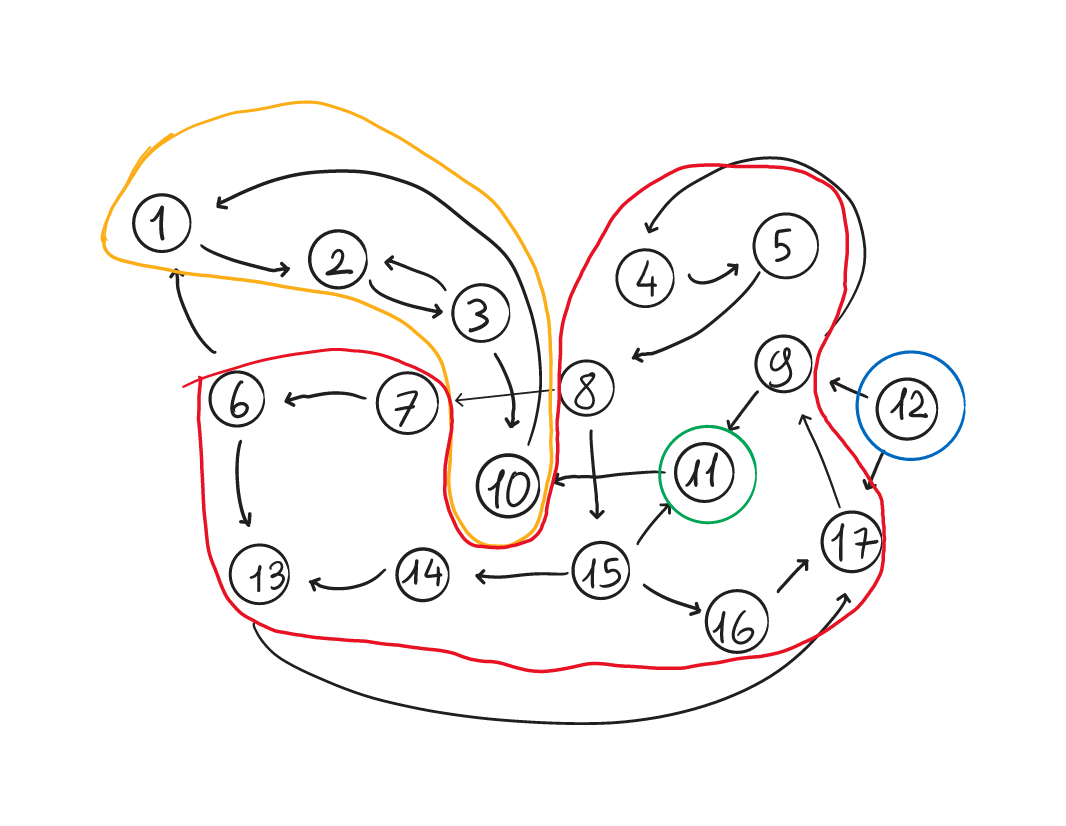
\includegraphics[width=\textwidth]{es1.png}
\begin{itemize}
    \item \textbf{\(SSC_1\):} \(\{1,2,3,10\}\)
    \item \textbf{\(SSC_2\):} \(\{4,5,6,7,8,9,13,14,15,16,17\}\)
    \item \textbf{\(SSC_3\):} \(\{11\}\)
    \item \textbf{\(SSC_4\):} \(\{12\}\)
\end{itemize}

\section{Esercizio 2}
\begin{enumerate}
    \item[A)] Dato un grafo \(G = (V, E)\) che rappresenta le amicizie su Facebook, prendendo due persone in \(V = FB\) \(p_1\) e \(p_2\) possiamo sempre individuare un \emph{path} da \(p_1\) a \(p_2\) di lunghezza \(\leq 6\)
    \item[B)] \[FB \times FB \subseteq \bigcup_{i = 1}^6 FBFriends^i\]
\end{enumerate}

\section{Esercizio 3}
\begin{align*}
     & R \cap R^{op} \subseteq Id_A                                                                                    & \text{\{Definizione di \(\subseteq\)\}} \\
     & \iff \forall (a,b) \in A \times A \text{ se } (a,b) \in R \cap R^{op} \text{ allora } (a,b) \in Id_A            & \text{\{Definizione di \(\cup\)\}}      \\
     & \iff \forall (a,b) \in A \times A \text{ se } (a,b) \in R \land (a,b) \in R^{op} \text{ allora } (a,b) \in Id_A & \text{\{Definizione di \(.^{op}\)\}}    \\
     & \iff \forall (a,b) \in A \times A \text{ se } (a,b) \in R \land (b,a) \in R \text{ allora } (a,b) \in Id_A      & \text{\{Definizione di \(Id\)\}}        \\
     & \iff \forall (a,b) \in A \times A \text{ se } (a,b) \in R \land (b,a) \in R \text{ allora } a = b               & \text{\{Definizione di anti-simm.\}}    \\
     & \iff \text{R è anti-simmetrica}
\end{align*}

\section{Esercizio 4}
L'enunciato è falso. Un controesempio è \\
\(A = \{a,b,c\}\)\\
\(R = \{(a,b), (b,c), (c,a)\}\)\\
\(R^* = \{(a,a), (b,b), (c,c), (a,b), (b,c), (c,a), (a,c), (c,b), (b,a)\}\)
\section{Esercizio 5}
\begin{enumerate}
    \item[a)] Falso. Un controesempio è il grafo \(G\) non riflessivo. \[G = (\{a,b,c\}, \{(a,b), (b,c)\})\]
    \item[b)] False. Un controesempio è il grafo \(G\) non transitivo. \[G = (\{a,b,c\}, \{(a,b), (b,c)\})\]
    \item[c)] Vero.
        Per dimostrare questo fatto dobbiamo dimostrare che \(E^*\) sia riflessiva, transitiva e anti-simmetria, dalla definizione di ordinamento parziale.
        \(E^*\) è la chiusura riflessiva e transitiva di \(E\), quindi per definizione è riflessiva e transitiva. \\
        Manca quindi da dimostrare che \(E^*\) sia anti-simmetrica, quindi l'implicazione
        \[(x,y), (y,x) \in E^* \implies x = y\]
        Prese due coppie del tipo \((x,y)\) e \((y,x) \in E^*\), per definizione di chiusura transitiva e riflessiva, se G è un DAG allora esiste un path da x a y, e viceversa.
        Quindi se \(x\) fosse diverso da \(y\) avremmo un ciclo da \(x\) a \(x\) e quindi G non potrebbe essere un DAG.

\end{enumerate}

\section{Esercizio 6}
\begin{enumerate}
    \item Vero. Ogni nodo sorgente per definizione avrà grado di ingresso uguale a 0. Quindi considerando il DAG \(H = (V, E^{op})\) abbiamo che tutti gli archi connessi ai nodi sorgenti sono invertiti, di conseguenza i nodi sorgenti avranno grado di uscita e entrata invertiti, quindi diventano pozzi.
    \item Vero. Stessa dimostrazione del punto 1, ma considerando i pozzi.
    \item Falso. Un controesempio è
          \[G = (\{a,b\}, \{(a,b)\}) \quad H = (\{a,b\}, \{(b,a)\})\]
    \item Vero. Se posso seguire gli archi in \(E\) per arrivare da \(y\) a \(x\) in \(H\), allora certamente posso seguire la stessa sequenza di archi invertiti in \(E^{op}\) per arrivare da \(x\) a \(y\) in G. \\
          Se esiste un walk da \(x\) a \(y\) in \(G\) ciò significa che posso seguire una sequenza di archi in \(E\) per arrivare da \(x\) a \(y\) in \(G\), allora certamente posso seguire la stessa sequenza di archi invertiti in \(E^{op}\) per arrivare da \(y\) a \(x\) in \(H\).
    \item Vero. G è DAG se e solo se \(E^*\) è ordinamento parziale, quindi mi basta dimostrare che \((E^{op})^*\) sia ordinamento parziale.\\
          Per la legge di distributività di * su \(.^{op}\)
          \[(E^{op})^* = (E^*)^{op}\]
          ma allora considerando che per ipotesi di DAG \(E^*\) è ordinamento parziale, devo dimostrare che la relazione opposta di \(E^*\) ordinamento parziale sia a sua volta ordinamento parziale. \\
          Considerando una relazione di ordinamento parziale, che quindi è riflessiva transitiva e anti-simmetrica, devo verificare che queste tre proprietà siano mantenute facendo la relazione opposta.
          \begin{itemize}
              \item Riflessività: invertendo le coppie del tipo \((a,a)\) ottengo esattamente le stesse coppie
              \item Transitività: prese due coppie qualsiasi \((a,b), (b,c)\) per transitività ho anche la coppia \((a,c)\). Ma invertendo tutte e tre le coppie, ottengo \((c,b), (b,a) e(c,a)\) quindi mantengo la transitività.
              \item Anti-simmetria: se la relazione non contiene coppie del tipo \((a,b), (b,a)\) con \(a \neq b\), allora invertendo tutti gli archi non potrò mai ottenere tali coppie.
          \end{itemize}
          Verificate queste proprietà, possiamo dire che \((E^*)^{op}\) è ordinamento parziale, e che quindi \((E^{op})^*\) è ordinamento parziale.
\end{enumerate}

\section{Esercizio 7}
\begin{enumerate}
    \item \(P(n): mult2(n,m) = mult2(n) + mult(m)\)\\
          Caso base: Per ogni \(m \in \mathbb{N}\) vale
          \begin{align*}
              P(0) & = mult2(0 + m)        &  & \{\text{calcolo}\}             \\
                   & = mult2(m)            &  & \{\text{calcolo}\}             \\
                   & = 0 + mult2(m)        &  & \{\text{clausola base mult2}\} \\
                   & = mult2(0) + mult2(m)
          \end{align*}
          Passo induttivo: Per ogni \(m \in \mathbb{N}\) vale
          \[\forall n \in \mathbb{N} \text{ vale che } P(n) \implies P(n+1)\]
          \begin{align*}
               & mult2(n + 1 + m) =        &  & \{\text{calcolo}\}                               \\
               & = mult2(n + m + 1) =      &  & \{\text{clausola induttiva mult2}\}              \\
               & = 2 + mult2(n + m) =      &  & \{\text{ipotesi induttiva}\}                     \\
               & = 2 + mult2(n) + mult2(m) &  & \{\text{clausola induttiva mult2 al contrario}\} \\
               & = mult2(n + 1) + mult2(m)
          \end{align*}

    \item \(Q(n): sum(n, f;mult2(n,m)) = mult2(sum(n,f))\)\\
          Caso base: Per ogni \(f \in Fun(\mathbb{N},\mathbb{N})\) vale \(Q(0)\)
          \begin{align*}
              sum(0,f;mult2) & = mult2(sum(0,f)) &  & \{\text{clausola base di sommatoria}\} \\
              (f;mult2)(0)   & = mult2(f(0))
          \end{align*}
          Passo induttivo: Per ogni \(f \in Fun(\mathbb{N},\mathbb{N})\) vale \(Q(n) \implies Q(n + 1)\)
          \begin{align*}
               & sum(n + 1,f;mult2)                                                        \\
               & = mult2(sum(n + 1, f))             &  & \{\text{clausola induttiva sommatoria}\} \\
               & = mult2(f(n+1) + sum(n,f))         &  & \{\text{P(n)}\}                          \\
               & = mult2(f(n+1)) + mutl2(sum(n,f))  &  & \{\text{ipotesi induttiva}\}             \\
               & = mult2(f(n+1)) + sum(n, f;mult2)  &  & \{\text{g(f(x)) = (f;g)(x)}\}            \\
               & = (f;mult2)(n+1) + sum(n, f;mult2) &  & \{\text{clausola induttiva sommatoria}\} \\
               & = sum(n + 1, f;mult2)
          \end{align*}
\end{enumerate}

\end{document}